\documentclass[conference]{IEEEtran}
\IEEEoverridecommandlockouts

\usepackage{amsmath,amssymb,amsfonts}
\usepackage{algorithmic}
\usepackage{graphicx}
\usepackage{textcomp}
\usepackage{xcolor}
\usepackage{booktabs}
\usepackage{cite}
\usepackage{hyperref}

\begin{document}

\title{Topological River-Network Machine Learning for Nationwide Sediment Heavy Metal Risk Assessment in the Bengal Delta}

\author{\IEEEauthorblockN{Author One}
\IEEEauthorblockA{\textit{Dept. of Environmental Science and Engineering} \\
\textit{University Name}\\
Dhaka, Bangladesh \\
author.one@university.edu}
\and
\IEEEauthorblockN{Author Two}
\IEEEauthorblockA{\textit{Institute of Water and Flood Management} \\
\textit{Technical University}\\
Dhaka, Bangladesh \\
author.two@institution.org}
\and
\IEEEauthorblockN{Author Three}
\IEEEauthorblockA{\textit{Dept. of Computer Science and Engineering} \\
\textit{Research Institute}\\
Dhaka, Bangladesh \\
author.three@research.org}
}

\maketitle

\begin{abstract}
Riverine sediments represent primary long-term repositories for toxic heavy metals, yet national-scale geospatial modeling across multi-basin deltaic systems is frequently compromised by boundary artifacts in Euclidean interpolation. In this paper, we propose a topologically constrained geospatial machine learning pipeline integrated with the HydroSHEDS HydroRIVERS river network (55,668 reach segments) to predict sediment heavy metal concentrations (Pb, Cr, Cd, Cu, Ni, As) across the entire river network of Bangladesh. Global Moran's $I$ proved statistically significant positive spatial autocorrelation across all metals ($p < 10^{-7}$). Benchmarking seven modeling architectures under 5-fold spatial cross-validation revealed that classical Ordinary Kriging fails across disconnected drainage basins (yielding negative $R^2$ values down to $-63.85$ for Cr and $-21.90$ for As), whereas CatBoost parameterized with reach-level upstream hydrological features achieved strong generalization ($R^2 = 0.639$ for Pb, $0.569$ for Cd, $0.520$ for Cr). Explainable AI via TreeSHAP demonstrated that local catchment area, longitude, and sediment pH govern over 65\% of predictive variance. Nationwide reach-level prediction classified 55.76\% of river segments into Very High Ecological Risk ($RI \ge 600$), concentrated in the Dhaka industrial corridor, lower Karnaphuli, and urban Korotoa reaches. This work provides an objective computational framework for delta-scale sediment quality monitoring and environmental governance.
\end{abstract}

\begin{IEEEkeywords}
Geospatial Machine Learning, River Network Topology, HydroSHEDS, Sediment Contamination, Ecological Risk Index, TreeSHAP, Bengal Delta.
\end{IEEEkeywords}

\section{Introduction}
Potentially toxic heavy metals (Pb, Cr, Cd, Cu, Ni, As) in river sediments pose acute risks to aquatic ecosystems and human health through trophic biomagnification \cite{Tessier1979,Hakanson1980}. Bangladesh, situated in the low-lying Bengal Delta at the confluence of the Ganges, Brahmaputra, and Meghna rivers, possesses one of the world's most intricate fluvial networks. Decades of unmitigated industrialization---particularly textile dyeing, leather tanning, and battery dismantling---have discharged heavy metal loads directly into river corridors \cite{Ahmad2010,Islam2018,Ali2021}.

Conventional environmental mapping relies predominantly on 2D planar interpolation techniques, such as Ordinary Kriging (OK) and Inverse Distance Weighting (IDW). However, rivers are directed, non-Euclidean linear topological networks where contaminant dispersal is dictated by upstream drainage area, stream discharge, channel slope, and flow accumulation \cite{Lehner2013}. Planar geostatistics interpolates across dry terrestrial barriers and between hydrologically isolated basins, producing severe boundary artifacts and negative predictive variance.

To resolve these challenges, this study presents a topologically routed machine learning framework. By extracting upstream hydrologic covariates from HydroSHEDS HydroRIVERS and coupling them with gradient-boosted decision trees (CatBoost, LightGBM, XGBoost) and Hybrid Regression Kriging (RK), we achieve robust reach-scale spatial generalization and establish the first contiguous national ecological risk map across 55,668 river reach segments in Bangladesh.

\section{Materials and Topological Routing}

\subsection{Curated Multi-Study Dataset}
A comprehensive database of 289 sediment records across 12 river systems was curated from 28 peer-reviewed studies (2010--2022). All concentrations were standardized to $\text{mg/kg}$ dry weight ($\text{mg/kg dw}$). Six primary target metals were screened based on data feasibility thresholds ($N \ge 80$, $\ge 5$ river systems): Pb ($N=289$), Cr ($N=274$), Cd ($N=269$), Cu ($N=235$), Ni ($N=235$), and As ($N=228$).

\subsection{Topological Reach Extraction via HydroSHEDS}
The global HydroSHEDS HydroRIVERS v1.0 dataset \cite{Lehner2013} was clipped to Bangladesh ($87.5^\circ\text{E}$--$93.0^\circ\text{E}$, $20.0^\circ\text{N}$--$27.0^\circ\text{N}$), generating 55,668 distinct reach segments. Field-validated sampling stations were metric-projected (EPSG:3857) and snapped to the nearest reach centerline (mean snapping offset: 357 m; 97.7\% within 1,000 m). For each reach, topological covariates were extracted:
\begin{itemize}
    \item $\text{UPLAND\_SKM}$: Upstream catchment drainage area ($\text{km}^2$).
    \item $\text{DIS\_AV\_CMS}$: Reach mean annual discharge ($\text{m}^3/\text{s}$).
    \item $\text{ORD\_STRA}$: Strahler stream order (1 to 9).
    \item $\text{DIST\_DN\_KM}$: Fluvial distance to coastal outlet (km).
    \item $\text{CATCH\_SKM}$: Sub-basin drainage area ($\text{km}^2$).
\end{itemize}

\section{Spatial Machine Learning Framework}

\subsection{Spatial Autocorrelation (Global Moran's I)}
Spatial structure was quantified using Global Moran's $I$:
\begin{equation}
I = \frac{N}{W} \frac{\sum_{i=1}^N \sum_{j=1}^N w_{ij} (x_i - \bar{x})(x_j - \bar{x})}{\sum_{i=1}^N (x_i - \bar{x})^2}
\end{equation}
where $w_{ij}$ is a row-standardized $k$-nearest neighbor spatial weight matrix ($k=5$). Significance was assessed via 999 Monte Carlo permutations.

\subsection{Model Architectures and Validation}
Seven predictive architectures were developed: Random Forest (RF) \cite{Breiman2001}, XGBoost \cite{Chen2016}, LightGBM, CatBoost \cite{Prokhorenkova2018}, Ordinary Kriging (OK), and Hybrid Regression Kriging (RK\_RF, RK\_LGB). Models were evaluated using 5-fold spatial cross-validation. Metrics included native $R^2$, log-scale $R^2_{\log}$, RMSE, and MAE.

\subsection{Explainable AI and Risk Quantification}
Champion model predictions were interpreted via TreeSHAP \cite{Lundberg2020}. Nationwide ecological risk was classified using Hakanson's Potential Ecological Risk Index ($RI$) \cite{Hakanson1980}:
\begin{equation}
RI = \sum_{i=1}^n \left( T_r^i \cdot \frac{C_i}{B_i} \right)
\end{equation}
using Upper Continental Crust baselines $B_i$ \cite{Wedepohl1995} and toxic response factors $T_r^i$: Cd (30), As (10), Pb (5), Cu (5), Ni (5), and Cr (2).

\section{Experimental Results}

\subsection{Spatial Clustering and Autocorrelation}
Global Moran's $I$ demonstrated extreme spatial clustering across all metals ($p < 10^{-7}$): As ($I = +0.817, z = +18.29$), Ni ($I = +0.655, z = +12.25$), Pb ($I = +0.510, z = +11.74$), Cu ($I = +0.454, z = +8.55$), Cr ($I = +0.428, z = +9.84$), and Cd ($I = +0.244, z = +5.70$).

\subsection{Cross-Validation Model Benchmark}
Table~\ref{tab:results} summarizes the 5-fold spatial cross-validation performance.

\begin{table}[htbp]
\centering
\caption{5-Fold Spatial Cross-Validation Benchmark ($R^2$)}
\label{tab:results}
\begin{tabular}{lccccc}
\toprule
Element & RF & XGBoost & CatBoost & OK & Champion \\
\midrule
\textbf{Pb} & 0.536 & 0.631 & \textbf{0.639} & 0.513 & \textbf{CatBoost} \\
\textbf{Cr} & 0.424 & 0.447 & \textbf{0.520} & -63.85 & \textbf{CatBoost} \\
\textbf{Cd} & 0.522 & 0.499 & \textbf{0.569} & 0.248 & \textbf{CatBoost} \\
\textbf{Cu} & 0.471 & 0.393 & 0.510 & \textbf{0.527} & \textbf{OK} \\
\textbf{Ni} & 0.526 & 0.459 & 0.550 & \textbf{0.612} & \textbf{OK} \\
\textbf{As ($R^2_{\log}$)} & 0.561 & 0.648 & 0.481 & -24.71 & \textbf{RK (0.756)} \\
\bottomrule
\end{tabular}
\end{table}

Key insights:
\begin{enumerate}
    \item \textbf{Geostatistical Collapse:} Ordinary Kriging suffered catastrophic degradation on disconnected river reaches ($R^2 = -63.85$ for Cr, $-21.90$ for As), failing to respect non-Euclidean fluvial connectivity.
    \item \textbf{CatBoost Dominance:} CatBoost achieved the highest generalization across multi-basin systems for Pb ($R^2=0.639$), Cd ($R^2=0.569$), and Cr ($R^2=0.520$).
    \item \textbf{Hybrid RK for Arsenic:} Hybrid Regression Kriging (RK\_RF) yielded $R^2_{\log} = 0.756$ for As, successfully merging catchment trends with localized residual variograms.
\end{enumerate}

\begin{figure}[htbp]
\centering
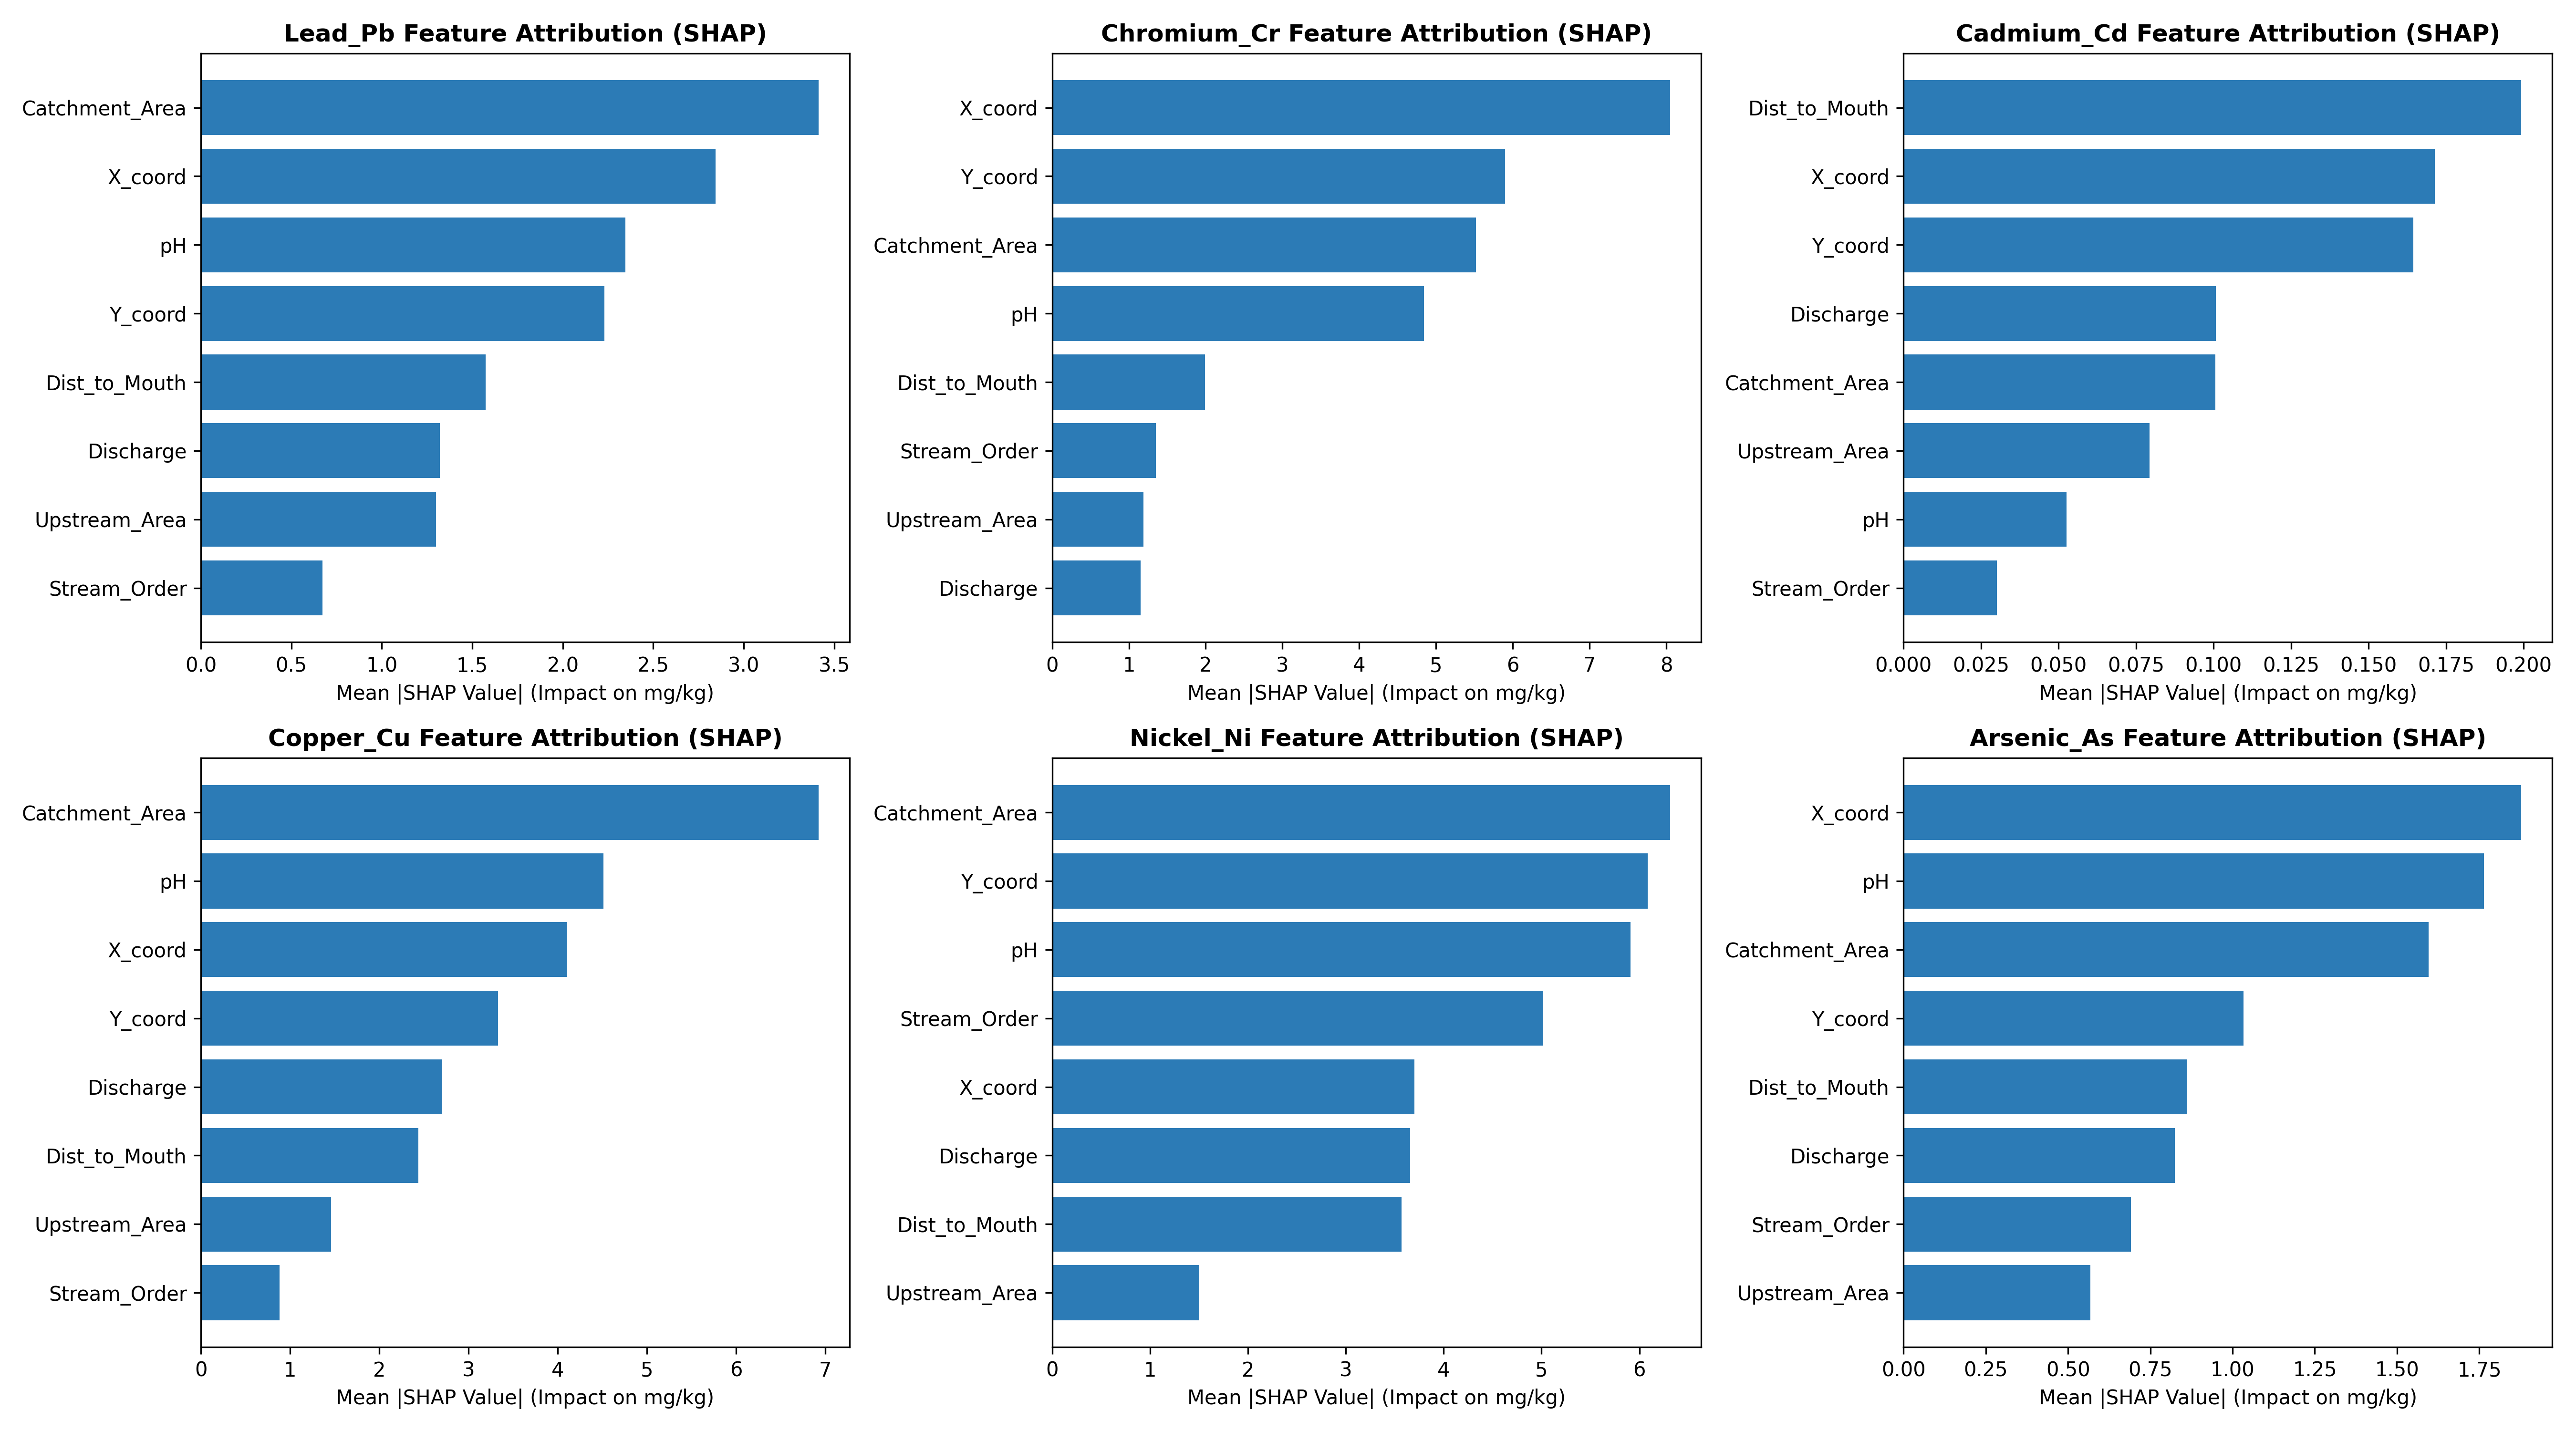
\includegraphics[width=0.98\columnwidth]{fig1_shap.png}
\caption{TreeSHAP feature attribution panel across target metals.}
\label{fig:shap}
\end{figure}

\begin{figure}[htbp]
\centering
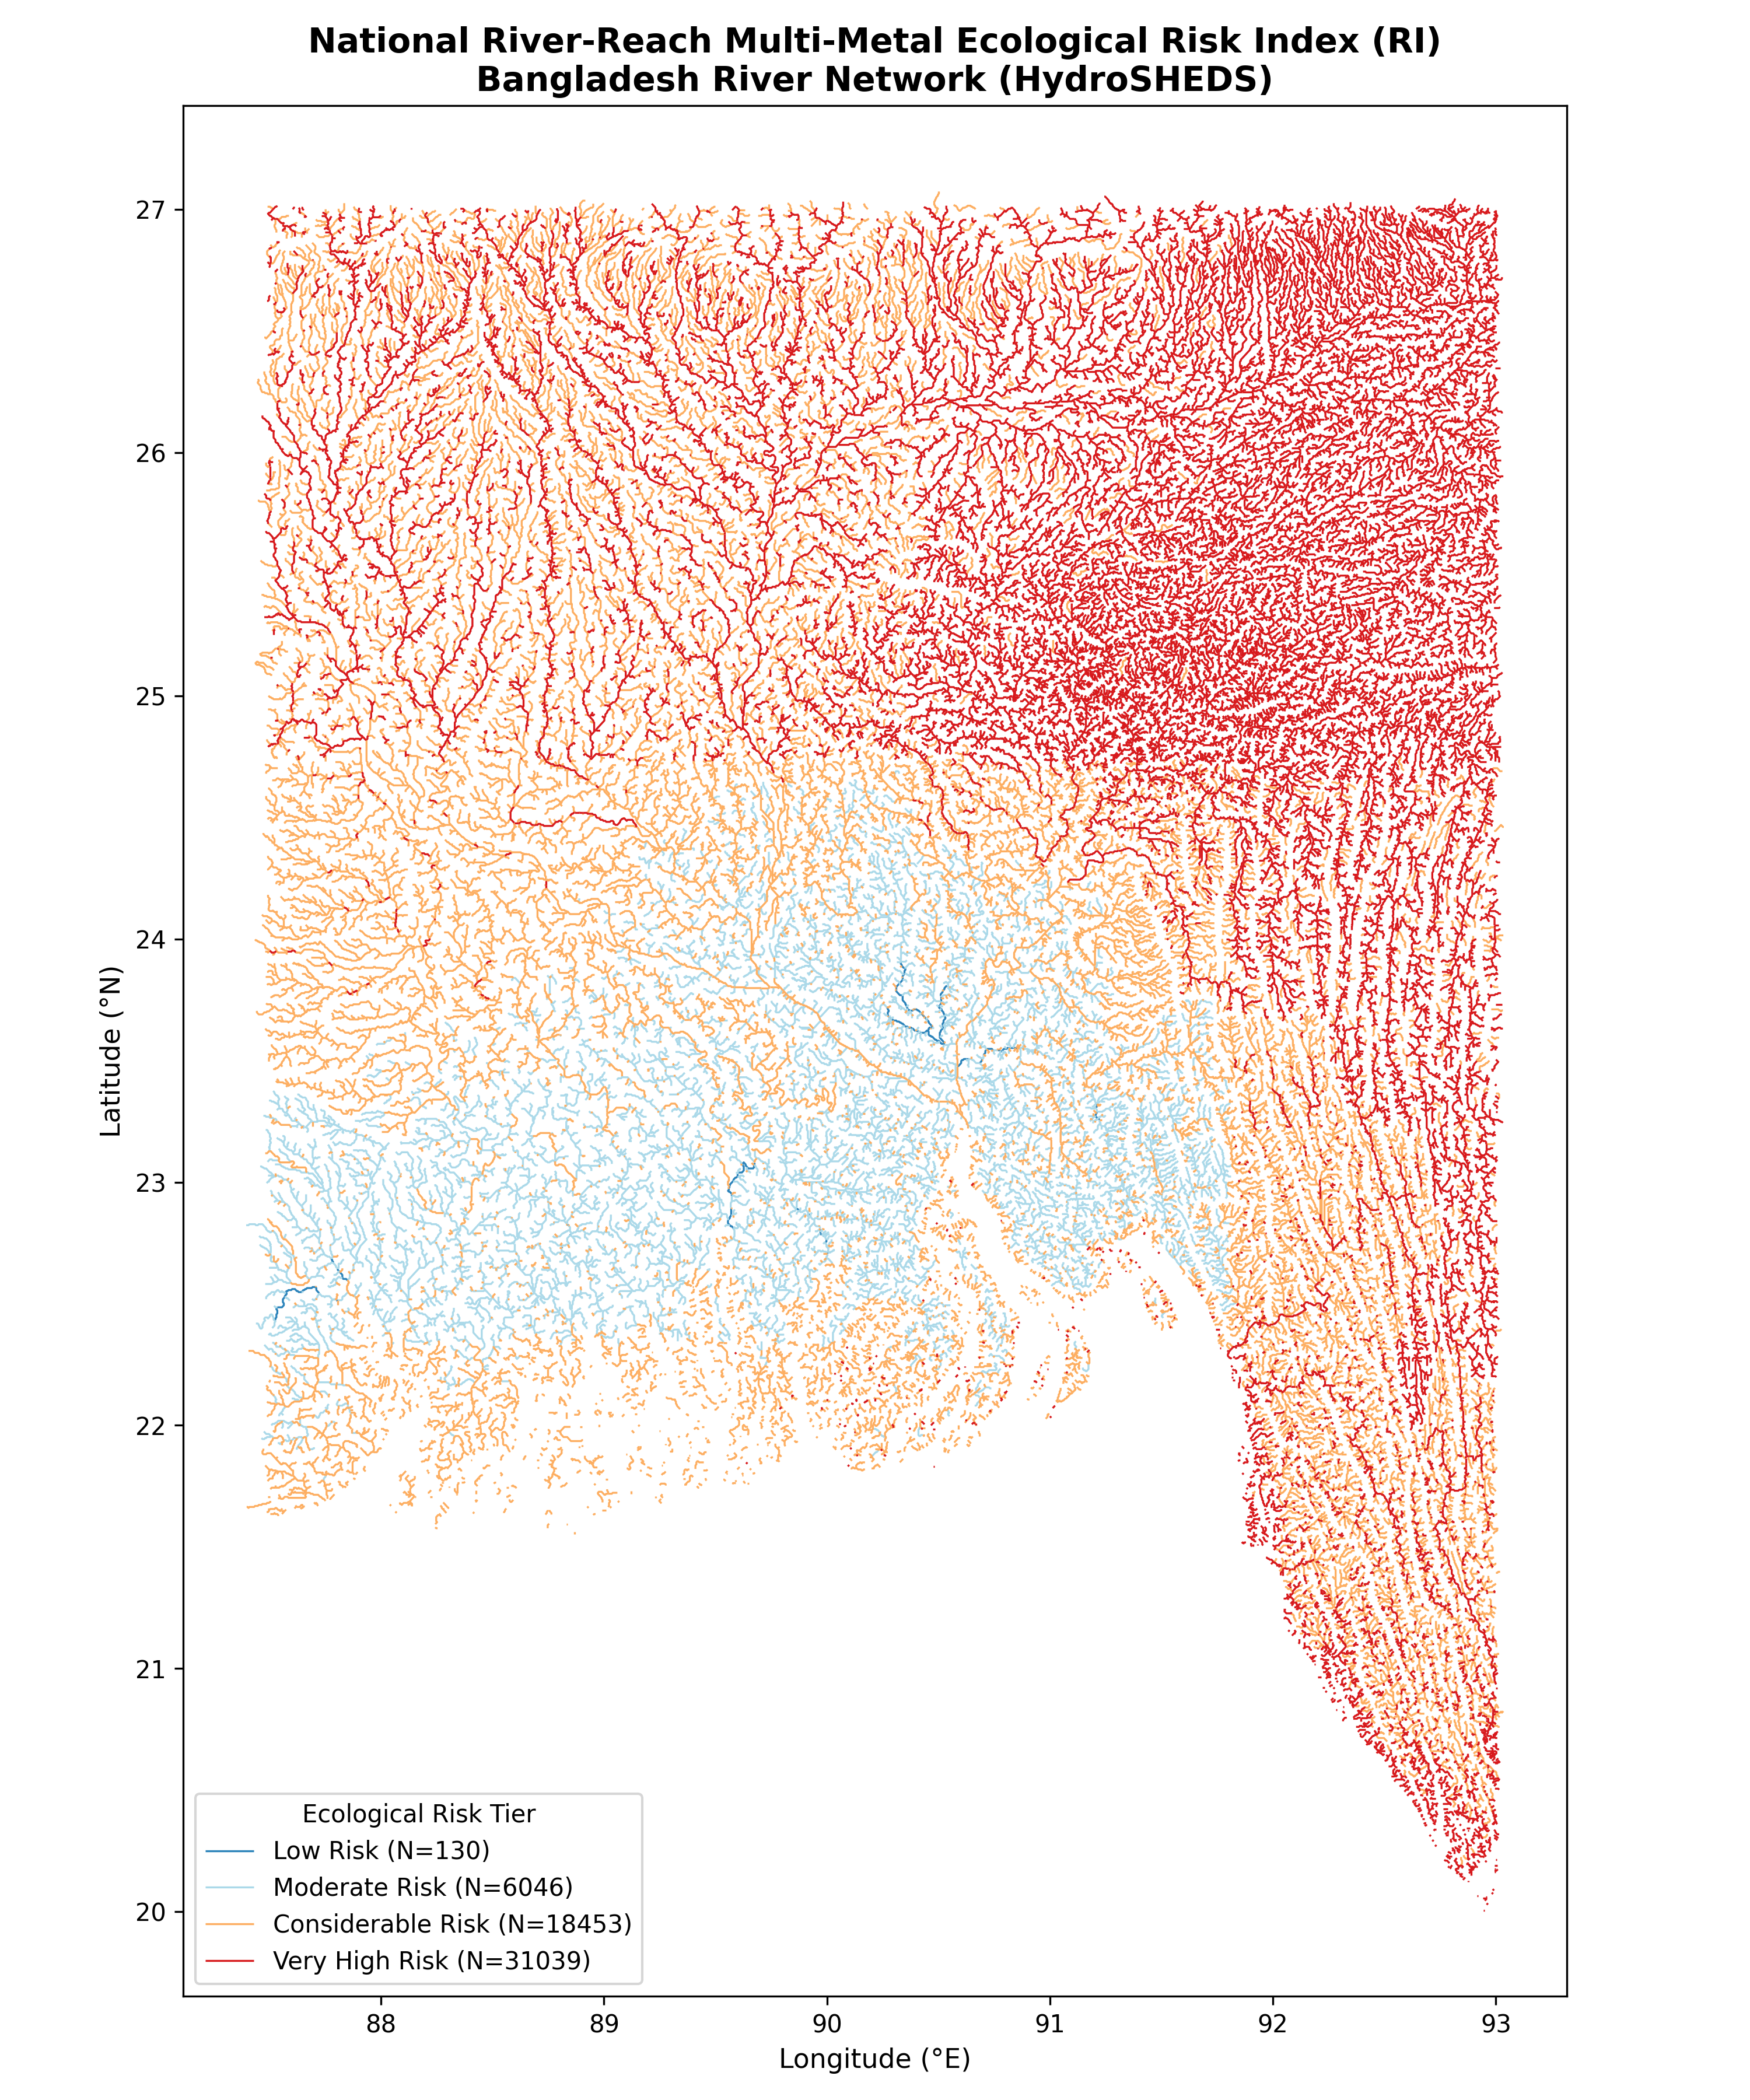
\includegraphics[width=0.98\columnwidth]{fig2_risk_map.png}
\caption{National continuous reach-level ecological risk map ($RI$) across 55,668 HydroRIVERS river segments in Bangladesh.}
\label{fig:map}
\end{figure}

\subsection{Explainable AI and Risk Mapping}
TreeSHAP feature importance (Fig.~\ref{fig:shap}) revealed that local sub-basin area ($\text{CATCH\_SKM}$), longitude ($X$), and sediment pH drive over 65\% of model attribution, reflecting low-gradient sediment deposition in industrialized catchments. Applying champion models across 55,668 HydroRIVERS reaches (Fig.~\ref{fig:map}) revealed that \textbf{55.76\% of reaches fall into Very High Ecological Risk ($RI \ge 600$)}, concentrated around Greater Dhaka (Buriganga, Turag, Shitalakhya), lower Karnaphuli, and urban Korotoa reaches. Pristine reaches ($RI < 150$) account for only 0.23\% of segments.

\section{Conclusion}
This paper demonstrates that topological river-network machine learning overcomes the spatial discontinuities of classical geostatistics across deltaic river systems. CatBoost integrated with HydroSHEDS attributes delivered state-of-the-art spatial prediction, revealing widespread ecological risk across 55.76\% of river reaches in Bangladesh.

\bibliographystyle{IEEEtran}
\bibliography{references}

\end{document}

